\section{Progettazione concettuale}
Il seguente schema ER è stato ottenuto seguendo una strategia \textbf{top-down}.

\subsection{Schema ER}
\begin{figure}[H]
    \centering
    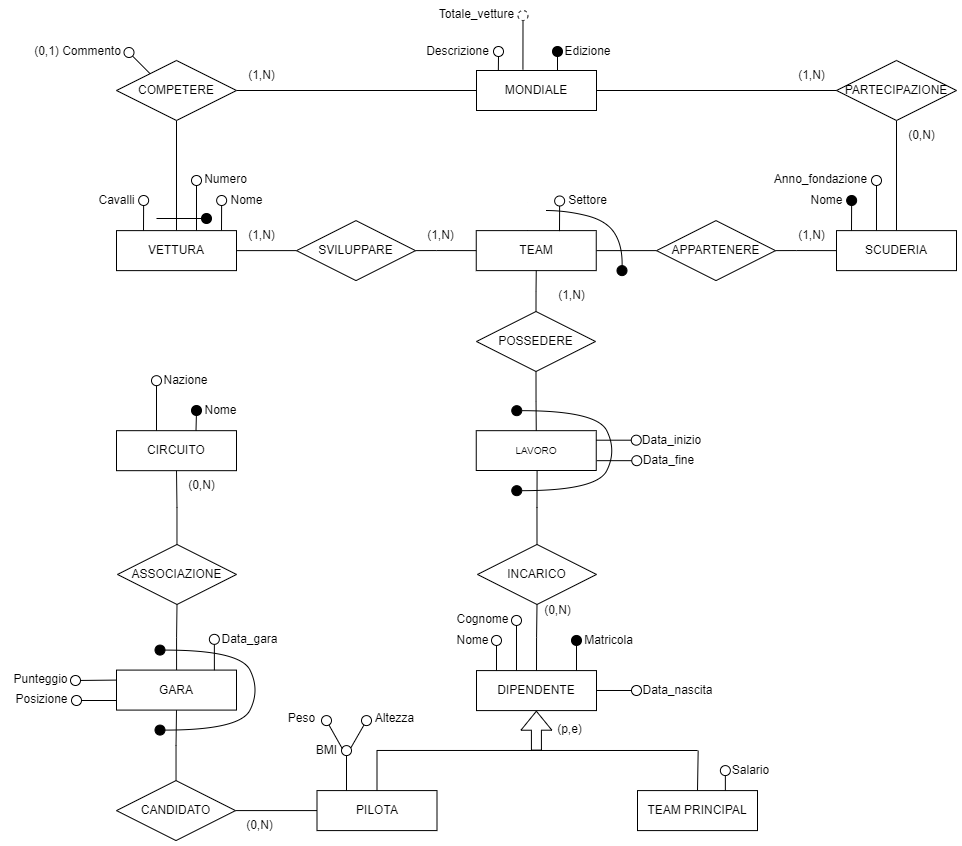
\includegraphics[scale = 0.73]{Images/ER.png}
\end{figure}

\newpage
\subsection{Business rules}
Passiamo adesso alla documentazione di supporto creando un'interpretazione personale dello schema e descrivendo le proprietà dei dati rappresentati.

\subsubsection{Descrizione dei concetti}

\begin{figure}[H]
    \centering
    \includegraphics[scale = 0.74]{Images/Table/Dizionario dei dati - entità dello schema.png}
\end{figure}


\begin{figure}[H]
    \centering
    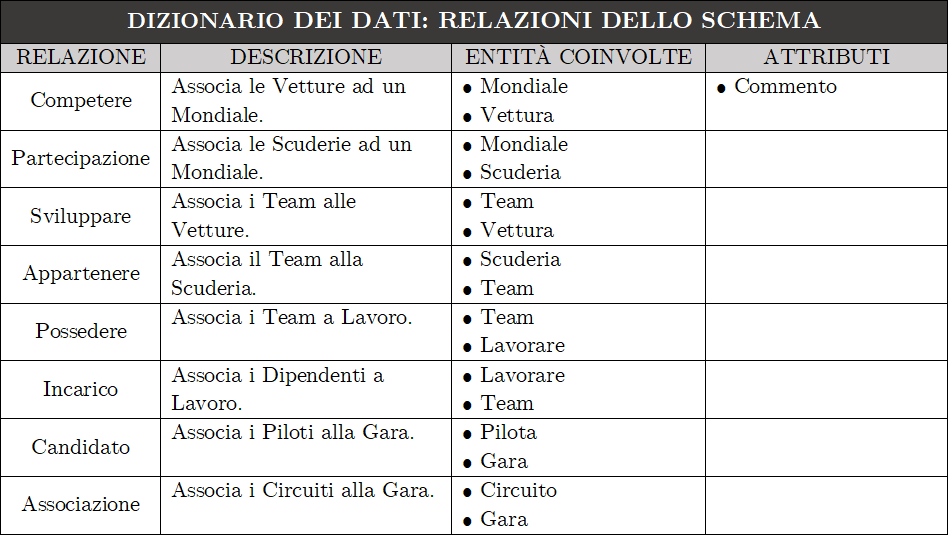
\includegraphics[scale = 0.74]{Images/Table/Dizionario dei dati - relazioni dello schema.png}
\end{figure}


\subsection{Vincoli d'integrità}
\begin{itemize}
    \item[$\diamondsuit$]  In un mondiale devono partecipare minimo 1 scuderia e massimo 10;
    \item[$\diamondsuit$] Una scuderia non deve partecipare allo stesso mondiale più di 1 volta;
    \item[$\diamondsuit$] Un team deve sviluppare minimo 1 vettura e 2 due;
    \item[$\diamondsuit$] Una vettura non deve partecipare a più di un mondiale;
    \item[$\diamondsuit$] Un pilota deve essere candidato ad almeno una gara;
    \item[$\diamondsuit$] In un circuito non devono esserci più gare nello stesso momento.
\end{itemize}

\subsection{Derivazioni}
\begin{itemize}
    \item[$\diamondsuit$] Il numero totale delle vetture che hanno partecipato ai mondiali si ottiene contando il numero di relazioni tra Mondiale e Vettura.
\end{itemize}

\subsection{Carico applicativo}

\subsubsection{Tavola dei volumi}
\begin{figure}[H]
    \centering
    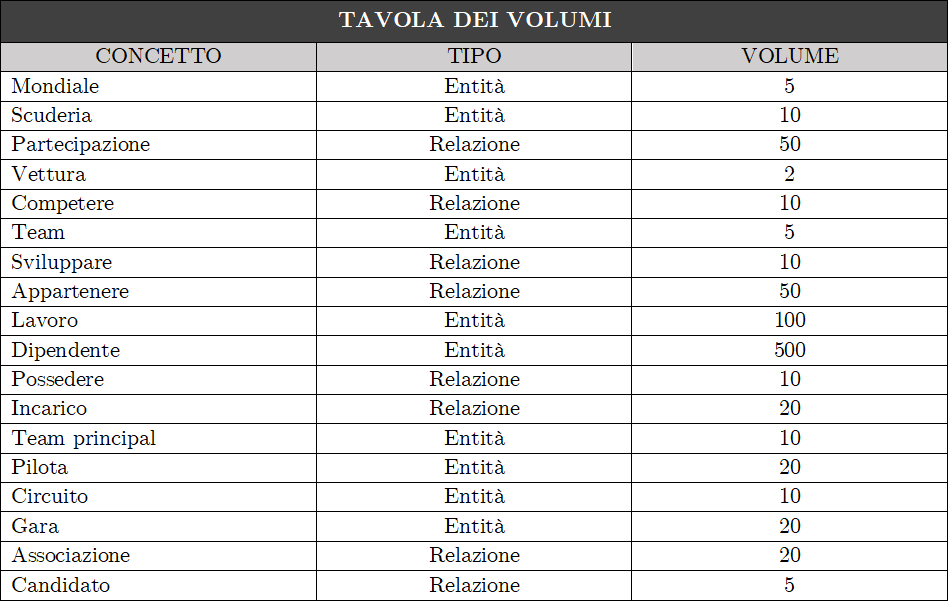
\includegraphics[scale = 0.74]{Images/Table/Tavola volumi.png}
\end{figure}

\subsubsection{Tavola delle operazioni}
\begin{figure}[H]
    \centering
    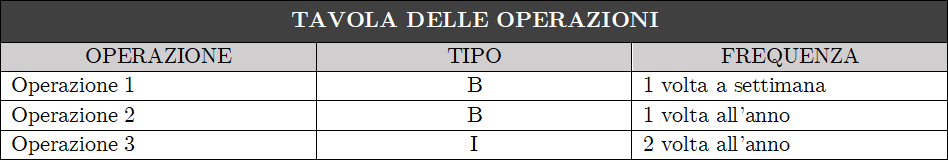
\includegraphics[scale = 0.74]{Images/Table/Tavola operazioni.png}
\end{figure}

\begin{itemize}
    \item \textbf{Operazione 1:} Generazione della classifica;
    \item \textbf{Operazione 2:} Visualizzazione del numero totale di macchine partecipanti al mondiale;
    \item \textbf{Operazione 3:} Inserimento di un nuovo circuito.
\end{itemize}

\subsubsection{Tavole degli accessi}

\begin{figure}[H]
    \centering
    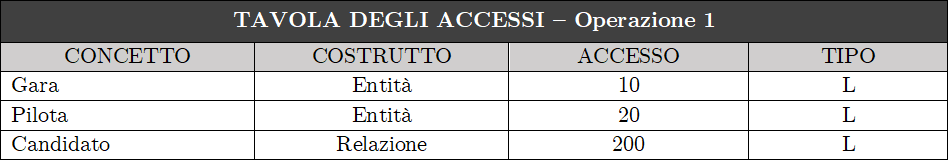
\includegraphics[scale = 0.74]{Images/Table/Tavola accessi - op1.png}
\end{figure}

\begin{equation*}
    230L \cdot 4 = 920L \cdot 12 = 11040L
\end{equation*}

In totale abbiamo 144 accessi annui il che potrebbe farci pensare di \emph{conservare}, creando un entità, la classifica all'interno del DataBase.

\begin{figure}[H]
    \centering
    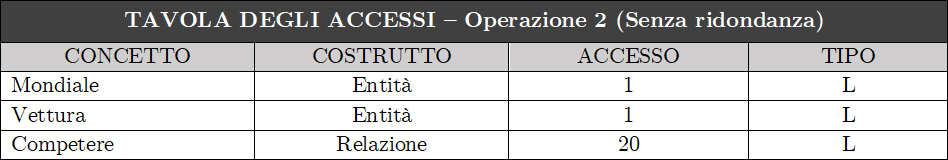
\includegraphics[scale = 0.74]{Images/Table/Tavola accessi - op2.png}
\end{figure}

\begin{equation*}
    22L
\end{equation*}

Passiamo adesso ad analizzare la tavola degli accessi mantenendo l'attributo \emph{Totale$\_$vetture} ridondante:

\begin{figure}[H]
    \centering
    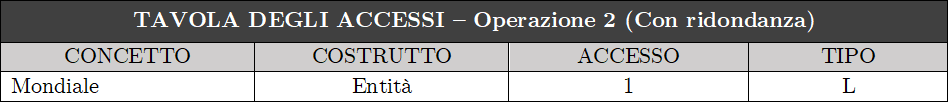
\includegraphics[scale = 0.74]{Images/Table/Tavola accessi - op2 (ridondanza).png}
\end{figure}

\begin{equation*}
    1L + 1Byte
\end{equation*}

Dall'analisi degli accessi si può notare come il mantenimento dell'attributo è conveniente e quindi si può lasciare all'interno dello schema.

\begin{figure}[H]
    \centering
    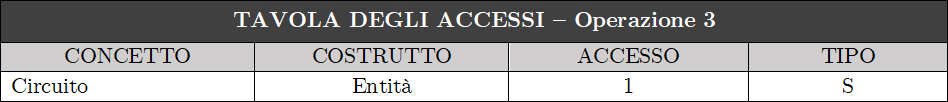
\includegraphics[scale = 0.74]{Images/Table/Tavola accessi - op3.png}
\end{figure}

\begin{equation*}
    1S = 2L
\end{equation*}